\section{\uppercase{Introduction}}
\label{sec:intro}

\noindent Electric vehicles are reaching end of life (EoL) in large numbers, and
the battery packs they carry are simultaneously a hazard and a source of critical
raw materials. Lithium, cobalt and nickel are all classified by the European
Commission as critical raw materials with elevated supply risk
\citep{eccrm,harper2019}, and European recycling capacity demand is projected to
reach 170\,GWh by 2035 \citep{te2024}. Regulation (EU) 2023/1542 additionally
requires documented condition data across the battery lifecycle
\citep{eubattreg}, which manual inspection delivers inconsistently.

Disassembly of EoL packs nevertheless remains predominantly manual. The
operation is labour intensive, slow, and exposes workers to high voltage and to
the risk of thermal runaway. A substantial research effort is consequently
directed at automating it \citep{zang2024robotic,tan2025screws}.

Every such system begins with perception. Before a manipulator can unfasten,
grasp or lift a component, the battery modules and the busbars that connect them
must be located in the image. The established approach is a supervised object
detector trained on imagery collected at a single facility or from a single
experimental rig. This practice conceals a problem specific to the application. A
recycling line does not receive a single pack type; it receives whatever arrives
on a given day, from different manufacturers, in different states of
disassembly, under whatever illumination the building provides. Accuracy
measured on the distribution a detector was trained on therefore carries limited
information about the next pack through the door.

To quantify this effect a cross-facility benchmark is required, and none exists
for the task. Every study surveyed in Section~\ref{sec:related} collected and
annotated its own imagery, and none released it. To address this gap, this paper
assembles a corpus of 4,425 training images from 13 independent public sources
spanning ten EV pack families, constructs a held-out cross-facility benchmark of
225 images containing 780 instances, and evaluates detectors on it under a single
harmonised protocol.

The principal finding is that the dominant failure mode in this setting is
neither image difficulty nor model capacity. It is disagreement between sources
about what the target class denotes. Per-source module accuracy across the
benchmark spans 0.995 to 0.043, and inspection confirms that the source on which
accuracy collapses annotates small internal sub-components as modules while every
other source annotates pack-level modules. The detector learned the majority
convention and applied it consistently, so the collapse constitutes a
disagreement about the target rather than a failure of perception.

This observation is developed into a screening procedure. The contributions of
this paper are as follows:

\begin{enumerate}
\item A cross-facility corpus and benchmark for EV battery module and busbar
detection, assembled from 13 independent public sources spanning ten pack families,
verified free of train-test leakage by perceptual hashing and released with a
per-source provenance and licence record.
\item A convention-consistency screening procedure that identifies
annotation-divergent sources from a single merged-corpus training run using a robust
outlier criterion on per-source disaggregated accuracy, together with a positive
control in which a consensus source relabelled to a sub-component convention is
recovered by the screen while no other source changes status.
\item A training-free variant of the same procedure, computed from annotation
geometry alone over 4,760 label files, which identifies the same source with no
training run and permits a corpus to be screened before a detector is trained.
\item An architecture comparison under a matched 60-epoch budget, establishing that
self-supervised pretraining is marginally \emph{worse} on conventionally annotated
packs, at 0.955 against 0.979, and substantially better under annotation shift, at
0.337 against 0.097, a factor of 3.5.
\item The finding that validation data drawn from a single divergent source
\emph{inverts} checkpoint selection rather than merely biasing it: the selected
checkpoint is worse than the fixed-budget final checkpoint by 0.235 mAP@50, a relative
loss of 51\%, with non-overlapping bootstrap intervals and an effect 80 times the
seed-to-seed spread.
\item Five negative results, covering open-vocabulary detection, automatic
relabelling, naive multi-source merging, synthetic augmentation and prolonged
fine-tuning of a pretrained model, each of which constrains the design space.
\end{enumerate}

\noindent\textbf{Relation to prior work by the same authors.} The single-source
specialist evaluated in this paper is the detector reported in
\citep{katiyar2026mvml}, which addressed detection and condition assessment at a
single facility using a CPU-deployable two-stage pipeline. That work could not test
cross-facility transfer, which is precisely the limitation the present paper
addresses. The corpus, the benchmark, both screening procedures and all evaluation
reported here are new, and the condition-assessment stage of the earlier work is
deliberately not revisited.

\section{\uppercase{Related Work}}
\label{sec:related}

\subsection{Perception for Battery Disassembly}

\noindent \citet{zang2024robotic} surveyed robotic EV battery
disassembly and concluded that the process remains predominantly manual, with
perception and task uncertainty identified as the principal obstacles. \citet{wegener2015} demonstrated that pack designs vary sufficiently
between manufacturers that fixed automation does not transfer, which is the
practical reason perception must generalise. However, that study addressed
mechanical disassembly sequencing and did not evaluate a perception component.

Most published perception work for this application targets fasteners rather than
components. \citet{screwrcnn2021} proposed a screw detection method
combining Faster R-CNN with rotation edge similarity, reporting improved
localisation of the screw axis. However, the method was validated on a single
collection of laboratory imagery. \citet{screwbatt2023} developed a
YOLOX-family detector for active screw detection in EV battery disassembly using
1,719 hand-annotated images. However, the dataset was not released and accuracy
was reported only in domain. \citet{screwcompare2026}
presented a comparison of YOLOv11 against Faster R-CNN for the same task, and
observed that the field is hampered by a lack of public datasets; the study
resorts to laptop screws as a proxy domain, which limits the conclusions that
transfer to battery imagery.

Module-level and busbar-level perception is comparatively under-explored. \citet{tan2025screws} developed a collaborative robot that unfastens and
collects screws by fusing vision with force and torque sensing, reporting above
90\% unfastening efficiency. However, the vision component operates on a single
fixed pack geometry, so the reported figure does not characterise transfer.
\citet{cvmodule2023} applied instance segmentation with point-cloud
registration in order to grasp busbars on an industrial module. However, the
approach is restricted to one module type and requires a reference model of that
type.

A recurring theme is data scarcity. Every study named above collected and
hand-annotated its own imagery, and none released it. That absence motivates the
benchmark presented in this paper.

\subsection{Cross-Dataset Evaluation}

\noindent Domain shift is a well-documented failure mode in visual recognition.
\citet{recht2019} demonstrated that classifiers which appear strong
on the original ImageNet test split lose accuracy on a replication set collected
by the same protocol. However, that study varied the sampling procedure while
holding the label taxonomy fixed. \citet{koh2021wilds} assembled the
WILDS benchmark of in-the-wild distribution shifts across ten application
domains, and established that standard training degrades substantially under
such shift. However, WILDS likewise holds the annotation protocol constant within
each dataset, whereas the corpus considered in this paper varies both the imaging
distribution and the annotation protocol between sources.

\citet{northcutt2021} demonstrated that pervasive label errors in
established test sets destabilise benchmark rankings, and estimated an average
label error rate of 3.4\% across ten widely used datasets. However, that work
treats label error as noise about an agreed target, whereas the failure
characterised here is systematic disagreement about what the target is. The
distinction is consequential for merged corpora: noise averages out with scale
whereas a divergent convention does not, and the proposed screening procedure
operationalises exactly that distinction.

\citet{penquitt2026} developed Rechecked, a modular framework combining automatic
label-error detection with crowd-sourced verification, and applied it to the
pedestrian class of KITTI, in which 18\% of the original ground-truth labels were
found to be missing or inaccurate. However, the framework corrects errors relative
to an annotation standard that is agreed within a single dataset, and the authors
report that the best available detection methods still miss up to 66\% of label
errors. The failure characterised in the present work is of a different kind: the
sources do not disagree about individual boxes, they disagree about what the class
denotes, and consequently no correction procedure operating within a single
convention can reconcile them. Section~\ref{sec:negative} reports an attempt at
exactly such a reconciliation, and its failure.

\citet{abouakar2026} investigated multi-source training for industrial object
detection, combining real imagery with rendered and generatively synthesised data,
and demonstrated that the composition of the training mixture materially affects
generalisation. However, the sources compared in that study share a single
annotation standard by construction, because the synthetic data is generated with
ground truth attached. The corpus considered here is multi-source in a stricter
sense, in that each contributing source carries an independently authored
annotation standard.

\subsection{Self-Supervised Representations for Detection}

\noindent Self-supervised backbones such as DINOv2 \citep{dinov2} learn features
that transfer without task-specific fine-tuning, and detection transformers
\citep{carion2020detr} initialised from them \citep{rfdetr} are reported to generalise better than
detectors trained from scratch in low-data regimes. However, that claim has been
established principally on natural imagery with a consistent annotation
protocol. Whether it holds on the cluttered, specular imagery of battery
internals, and whether it holds under annotation shift specifically, is evaluated
in Section~\ref{sec:res-arch}.

\subsection{Open-Vocabulary Detection and Automatic Annotation}

\noindent Open-vocabulary detectors such as YOLO-World \citep{yoloworld} and
Grounding DINO \citep{groundingdino} localise objects specified by free-text
prompts and have been proposed as a route to annotation-free deployment and to
automatic pre-annotation. However, their accuracy depends on the target concept
being represented in the vision-language pre-training corpus. The behaviour of
both on battery internals is reported in Section~\ref{sec:negative}.

Benchmark design for industrial vision has precedent outside this application.
\citet{bergmann2019mvtec} introduced MVTec AD, which established that a carefully
constructed benchmark with documented acquisition conditions can redirect an entire
sub-field. However, MVTec AD was collected by one group under controlled conditions
and therefore does not exhibit the inter-source annotation disagreement examined
here. \citet{zhou2022dg} surveyed domain generalisation methods and organised them
into data manipulation, representation learning and learning strategy. However, that
taxonomy presumes a fixed label space across domains, which is the assumption the
present work shows to fail on assembled corpora.

To the best of our knowledge, no public cross-facility benchmark for EV battery
component detection exists, and no prior study has quantified the contribution of
annotation-convention divergence to cross-source detection accuracy. Therefore,
this research presents both.

\section{\uppercase{Corpus and Benchmark}}
\label{sec:data}

\subsection{Sources}

\noindent A corpus of 4,425 training images was assembled from 13 independent
public sources spanning ten EV pack families, annotated with two classes,
\texttt{module} and \texttt{busbar}. Table~\ref{tab:sources} presents the
principal sources with their image counts and pack families.

The images and the polygon annotations originate with those sources. The
contribution made in this paper is the assembly, the deduplication, the audit and
the benchmark construction, not the annotation itself. Licences differ across
sources and one is non-commercial, so per-source provenance is recorded and
released so that any single source can be excluded by a downstream user.

\begin{table}[t]
\caption{Principal corpus sources. Thirteen sources in total, spanning ten EV
pack families.}
\label{tab:sources}
\centering
\begin{tabular}{lrl}
\hline
Source & Images & Pack family \\
\hline
ev-battery-comp-det. & 1,045 & multi-manufacturer \\
ev-battery-components & 680 & Audi / BMW / Chevrolet \\
last\_exp4 & 483 & multi-manufacturer \\
ev-battery-pack & 435 & single laboratory rig \\
battery\_comp & 280 & Nissan Leaf \\
ue\_d1\_defect & 237 & module close-ups \\
final\_mobilenet & 216 & multi-manufacturer \\
automated-disassembly & 117 & disassembly cell \\
bmw\_i3 & 111 & BMW i3 \\
ue\_rav4 & 96 & Toyota RAV4 \\
Others (three sources) & 725 & mixed \\
\hline
\end{tabular}
\end{table}

\subsection{Deduplication and Leakage Control}

\noindent Reported accuracy is informative only against a benchmark that does not
overlap the training data. All 4,440 candidate images were therefore compared by
difference hashing (dHash) at a Hamming distance threshold of 6. That threshold
was selected because it separates augmentation-derived near-duplicates from
genuinely distinct frames on this corpus; values below 4 admitted rotated
duplicates and values above 8 rejected distinct frames of the same pack.

Fifteen same-source near-duplicates were removed. A subsequent cross-source pass
at a looser threshold returned zero duplicates, which confirms that the sources
are genuinely independent collections rather than republications of one another.

This control proved necessary rather than precautionary. One candidate source, a
712-image public collection covering 19 vehicle types, republishes imagery from
another source already present in the corpus: 78 of its images were
byte-identical duplicates of training images, a fact stated in its own
documentation but easily overlooked. Merging without verification would have
placed training images directly into the benchmark and inflated every subsequent
measurement.

\subsection{Annotation Audit}
\label{sec:audit}

\noindent All 4,425 training images were audited for label and image quality.
Table~\ref{tab:audit} presents the outcome. Of the corpus, 23.5\% carries no
labels, 12.3\% scores low on a Laplacian-variance blur metric, 20.4\% is
greyscale, and no image contains a degenerate box.

\begin{table}[t]
\caption{Annotation and image-quality audit of the 4,425-image training corpus.}
\label{tab:audit}
\centering
\begin{tabular}{lrl}
\hline
Flag & Share & Assessment \\
\hline
Unlabelled & 23.5\% & partly harmful \\
Low blur score & 12.3\% & benign \\
Greyscale & 20.4\% & benign \\
Degenerate boxes & 0.0\% & --- \\
\hline
Polygon annotations & 86.8\% & 16,945 of 19,522 \\
\hline
\end{tabular}
\end{table}

Two findings changed how the corpus was treated. Firstly, the blur and greyscale
flags are largely false alarms. The lowest-scoring images are smooth, closed pack
lids, for which a Laplacian-variance metric reads flat metal as blurred, and the
greyscale images originate entirely from two monochrome sources. Both categories
add useful variation to the corpus, so deletion on the metric alone would degrade
it.

Secondly, the harmful category is unlabelled images that nonetheless contain
visible components. A proportion of the 23.5\% is legitimate background imagery,
which is beneficial in moderation because it suppresses false positives. However,
inspection confirmed open packs with clearly visible busbar assemblies carrying
no annotations at all. Such frames actively teach the detector that busbars are
background, and they are a plausible contributor to the weak busbar accuracy
reported in Section~\ref{sec:res-arch}.

The audit also established that 16,945 of the 19,522 annotations are polygon
masks, with between 5 and 151 vertices, rather than axis-aligned boxes. These are
converted to enclosing boxes for detection training and evaluation. It should be
noted that an early version of the evaluation pipeline silently discarded every
polygon-format label, trained on 20\% of the available annotations, and produced
an inflated score that appeared plausible on inspection. The failure is easy to
introduce and difficult to detect, and ground-truth instance counts should be
reconciled across pipelines as a matter of routine.

\subsection{The Cross-Facility Benchmark}

\noindent A cross-facility benchmark of 225 images containing 780 instances was
drawn from all sources and held out entirely from training. A convention-
consistent subset of 177 images, obtained by applying the screening procedure of
Section~\ref{sec:screen}, is reported alongside the full benchmark throughout
Section~\ref{sec:results}.

\section{\uppercase{Method}}
\label{sec:method}

\subsection{Detectors and Training Configurations}

\noindent Three configurations are compared.

The \emph{single-source specialist} is a YOLOv8n detector trained only on the
single-laboratory source at an input resolution of 768\,px, following the
conventional approach in this literature and reproducing the setting under which
published accuracy figures for this task are typically obtained.

The \emph{multi-source YOLO11n} configuration \citep{yolo11} comprises 2.6\,M
parameters and was trained from COCO initialisation \citep{lin2014coco} on all 13
sources at 640\,px with stochastic gradient descent.

The \emph{multi-source RF-DETR} configuration \citep{rfdetr} is a real-time detection
transformer initialised from the published RF-DETR-Nano checkpoint, whose backbone
derives from self-supervised DINOv2 pretraining \citep{dinov2}, fine-tuned end to end
on the same data at 672\,px. All 30.6\,M parameters are updated; the backbone is not
frozen.

\textbf{Matched training budget.} An architecture comparison is meaningful only when
both models receive equivalent training. Both multi-source configurations are
therefore trained for exactly 60 epochs, at the closest input resolutions the two
architectures accept, since RF-DETR requires a multiple of 56 and 672 is the nearest
such value to 640. Early stopping is disabled and the final checkpoint is taken, for
the reason established in Section~\ref{sec:res-inversion}: the validation data
available for this corpus is drawn from a single source, and selecting an epoch
against it inverts the ordering of checkpoints. YOLO11n was trained with three random
seeds; RF-DETR was trained once at the full budget, a limitation stated in
Section~\ref{sec:limits}.

\subsection{Harmonised Evaluation Protocol}

\noindent Confidence scores are not comparable across architectures, and mixing
metric implementations produced a spurious result in early experiments conducted
for this study. Every model is therefore scored with a single metric
implementation, at a common confidence threshold of 0.05, on identical images,
against identical ground truth including polygon-derived boxes. The threshold of
0.05 was selected because it lies below the operating point of all three
detectors and therefore does not truncate the precision-recall curve for any of
them.

\subsection{Convention-Consistency Screening}
\label{sec:screen}

\noindent The proposed screening procedure identifies sources whose annotation
convention diverges from the corpus consensus, using a single merged-corpus
training run and no additional annotation.

Let $\mathcal{S}=\{S_1,\dots,S_n\}$ denote the sources contributing to the
benchmark, and let $a_i$ denote the class-specific mAP@50 obtained by the
merged-corpus detector on the held-out images of source $S_i$. A source is
flagged as convention-divergent when its accuracy falls below a robust lower
fence, which is defined as follows:
\begin{equation}
a_i < \operatorname{med}(\mathbf{a}) - k \cdot c \cdot \operatorname{mad}(\mathbf{a}),
\label{eq:screen}
\end{equation}
where $\mathbf{a}=(a_1,\dots,a_n)$ denotes the vector of per-source accuracies,
$\operatorname{med}$ denotes the median, $\operatorname{mad}$ denotes the median
absolute deviation, $c=1.4826$ rescales the median absolute deviation to a
consistent estimator of the standard deviation under normality
\citep{rousseeuw1993mad}, and $k$ denotes a sensitivity parameter. A value of
$k=3$ is used throughout, which is the conventional choice for outlier rejection
and which is shown in Section~\ref{sec:res-screen} to separate the divergent
source from the consensus by a wide margin on this corpus.

The median and the median absolute deviation are used in place of the mean and
the standard deviation because a divergent source inflates both of the latter and
thereby partially masks itself. Consequently, the proposed procedure remains
sensitive when the divergent source is large, which is the case on this corpus.

Two practical conditions apply. Firstly, a source must contribute enough instances
for its accuracy to be estimated stably; a floor of 100 module instances is used
throughout, below which a source is excluded from the screen rather than reported. An
earlier evaluation at 40 instances produced a swing of 0.36 mAP@50 on the smallest
source between two models that differed only in the labels of an unrelated source,
which is sampling noise rather than signal. Secondly, the screen is computed on a
stratified sample of the corpus itself rather than on held-out data, because it is a
curation diagnostic and not a generalisation measure: a source whose labels
contradict the majority convention is not fitted well even during training. Absolute
values are consequently optimistic and only the relative ordering is used.

A source flagged by the proposed procedure is not discarded from the corpus. It
is reported separately as an out-of-convention benchmark, on the grounds
established in Section~\ref{sec:res-screen} that its labels encode a different
task rather than a degraded version of the same one. The procedure requires no
additional annotation, no additional training run beyond the merged-corpus model
that is trained in any case, and no prior assumption about which source is
divergent.

\subsection{Training-Free Screening from Annotation Geometry}
\label{sec:screen-free}

\noindent The procedure of Section~\ref{sec:screen} requires a merged-corpus
training run. A cheaper variant operates on the annotation files alone, which
permits a corpus to be screened before any detector is trained.

A source that annotates sub-components rather than pack-level modules produces many
small boxes per image, whereas a source following the consensus convention produces
few large ones. That signature is captured by a granularity index, which is defined
as follows:
\begin{equation}
g_i = \frac{n_i}{s_i},
\label{eq:granularity}
\end{equation}
where $n_i$ denotes the mean number of module instances per image in source $S_i$
and $s_i$ denotes the median normalised module scale, taken as the square root of
the enclosing-box area in normalised image coordinates. Scale is expressed as a
square root so that the index is dimensionally a count per unit length and is
therefore invariant to image resolution. The robust criterion of
Equation~\ref{eq:screen} is then applied to $\mathbf{g}$ with the inequality
reversed, since convention divergence raises the index rather than lowering it.

\section{\uppercase{Results}}
\label{sec:results}

\subsection{The Single-Source Evaluation Gap}
\label{sec:res-gap}

\noindent Table~\ref{tab:gap} quantifies the motivating problem. The specialist attains
0.818 mAP@50 on the single-source benchmark on which it was trained and validated, and
0.277 on a cross-facility benchmark drawn from all sources, a relative loss of 66\%.
Its in-domain accuracy therefore does not predict behaviour elsewhere.

\begin{table}[t]
\caption{Single-source against cross-facility accuracy for the specialist detector,
mAP@50.}
\label{tab:gap}
\centering
\begin{tabular}{lcc}
\hline
Model & In-domain & Cross-facility \\
\hline
Single-source specialist & \textbf{0.818} & 0.277 \\
\hline
\end{tabular}
\end{table}

It should be noted at the outset that the in-domain benchmark here is itself the
source whose annotation convention is shown below to diverge from the corpus
consensus. The figure therefore conflates generalisation loss with the specialist
having been trained on an idiosyncratic convention, and it is read as an upper bound
on the generalisation component rather than as a measurement of it. The remaining
results do not depend on it.

\subsection{Per-Source Screening}
\label{sec:res-screen}

\noindent The merged-corpus detector was evaluated per source on a stratified sample
of 1,628 images spanning 11 sources, using the procedure and instance floor of
Section~\ref{sec:screen}. Figure~\ref{fig:screen} presents the outcome. Accuracy on
six sources lies between 0.941 and 1.000, falls to 0.641 on one source and collapses
to 0.097 on another. Applying Equation~\ref{eq:screen} with $k=3$ yields a lower
fence of 0.864, and two sources fall below it.

\begin{figure}[t]
\centering
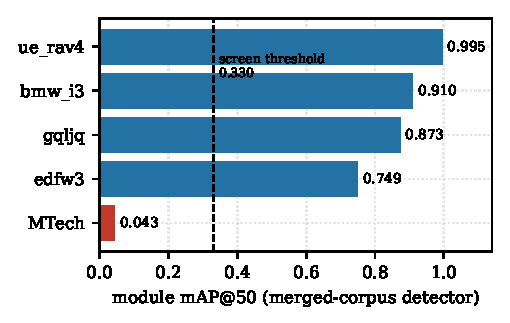
\includegraphics[width=0.98\columnwidth]{figures/fig_screen.pdf}
\caption{Per-source module accuracy for the merged-corpus detector, with the robust
lower fence of Equation~\ref{eq:screen} at $k=3$. Two sources fall below the fence,
one of them by a wide margin.}
\label{fig:screen}
\end{figure}

The two flagged sources differ in character. The source at 0.097 lies 0.767 below the
fence, an order of magnitude below the consensus band. Visual inspection confirms the
diagnosis: it annotates small internal sub-components in extreme macro views as
modules, whereas every other source annotates pack-level modules. The detector learned
the majority convention and applied it consistently, so the collapse constitutes a
disagreement about the target rather than a failure of perception. The source at
0.641 lies 0.223 below the fence and is a milder case; its granularity index in
Section~\ref{sec:res-screen-free} is the second highest in the corpus but does not
exceed the training-free fence, so the two screens disagree about it. That
disagreement is informative, and indicates the model-based screen to be the more
sensitive of the two.

Three sources were excluded for contributing fewer than 100 module instances. One of
these annotates busbars exclusively and contributes no module instances at all, a
fact the screen surfaces without any manual inspection.

\subsection{Training-Free Screening}
\label{sec:res-screen-free}

\noindent Equation~\ref{eq:granularity} was evaluated over all 4,760 label files in
the corpus, using no images and no trained model. The divergent source attains a
granularity index of 40.7, against 15.0 for the next highest source and a median of
9.00 across the corpus. Applying the robust criterion with $k=3$ yields an upper
fence of 29.02, and exactly one source exceeds it.

The source identified is the same one the model-based procedure flags most strongly.
The two screens are methodologically independent: one measures how a trained detector
behaves on images of each source, and the other measures only the geometry of the
annotations, with no model involved. Their agreement provides a second and
independent line of evidence that the source encodes a different annotation
convention rather than presenting harder imagery.

The practical implication is that a corpus may be screened before a detector is
trained. It should be noted that the training-free index detects divergence in
annotation \emph{granularity} specifically, which is the form present in this corpus.
Conventions that disagree about class boundaries while preserving object scale, for
example a source that labels a cooling plate as a module, would not be separated by
Equation~\ref{eq:granularity} and would still require the model-based procedure.

\subsection{Positive Control}
\label{sec:res-control}

\noindent Both screens were applied to a corpus in which the divergent source was
identified after the fact, so neither has been tested against a case whose answer is
known in advance. To supply one, a controlled positive was constructed. A consensus
source was relabelled to a deliberately different convention, in which every
pack-level module box is replaced by a $3\times2$ grid of inset sub-component boxes
covering the same region, imitating the granularity of the real divergent source. No
image is altered and no busbar annotation is touched, so any screen responding to the
manipulation responds to annotation convention and to nothing else. A detector was
then retrained on the manipulated corpus under the identical budget.

Table~\ref{tab:control} and Figure~\ref{fig:control} present the outcome. The
manipulated source falls from 0.941 to 0.667 and crosses the fence, while no
unmanipulated source moves by more than 0.050 and four move by 0.017 or less. The
flagged set gains exactly one member and loses none. On the training-free index the
same source rises from 11.1, inside the consensus band, to 185.8. Both screens
therefore recover a divergence whose ground truth is known by construction, without
producing false positives elsewhere.

\begin{table}[t]
\caption{Positive control. A consensus source is relabelled to a sub-component
convention and the detector is retrained. Values are module mAP@50 for the
model-based screen and the granularity index for the training-free screen.}
\label{tab:control}
\centering
\begin{tabular}{lccc}
\hline
Source & Original & Manipulated & Change \\
\hline
\multicolumn{4}{l}{\emph{model-based screen, fence 0.864 / 0.815}} \\
battery\_comp & 1.000 & 1.000 & $0.000$ \\
edfw3 & 0.982 & 0.973 & $-0.009$ \\
bmw\_i3 & 0.967 & 0.950 & $-0.017$ \\
\textbf{manipulated} & \textbf{0.941} & \textbf{0.667} & $\mathbf{-0.274}$ \\
automated & 0.641 & 0.591 & $-0.050$ \\
divergent & 0.097 & 0.097 & $0.000$ \\
\hline
\multicolumn{4}{l}{\emph{training-free screen, fence 29.02 / 35.24}} \\
\textbf{manipulated} & \textbf{11.1} & \textbf{185.8} & $\mathbf{+174.7}$ \\
\hline
\end{tabular}
\end{table}

\begin{figure*}[t]
\centering
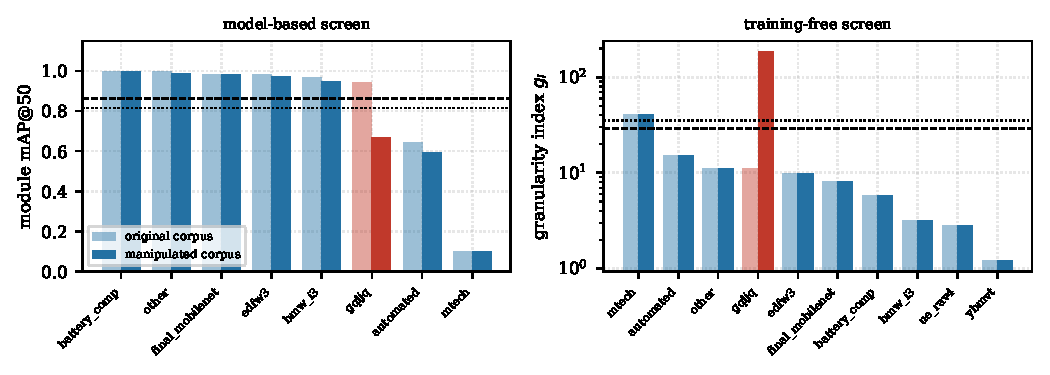
\includegraphics[width=0.86\textwidth]{figures/fig_control.pdf}
\caption{Positive control on both screens. Pale bars are the original corpus, solid
bars the corpus in which one consensus source has been relabelled to a sub-component
convention. Dashed and dotted lines are the robust fences before and after
manipulation. The manipulated source is the only one whose flag status changes.}
\label{fig:control}
\end{figure*}

\subsection{Architecture Comparison under a Matched Budget}
\label{sec:res-arch}

\noindent Both multi-source configurations were trained for 60 epochs and scored per
source under the identical protocol. Table~\ref{tab:arch} and Figure~\ref{fig:arch}
present the comparison.

\begin{table}[t]
\caption{Architecture comparison under a matched 60-epoch budget, module mAP@50.
Consensus is the mean over the six sources above the fence.}
\label{tab:arch}
\centering
\begin{tabular}{lccc}
\hline
Model & Consensus & Mild outlier & Divergent \\
\hline
YOLO11n & \textbf{0.979} & 0.641 & 0.097 \\
RF-DETR & 0.955 & \textbf{0.779} & \textbf{0.337} \\
\hline
\end{tabular}
\end{table}

\begin{figure}[t]
\centering
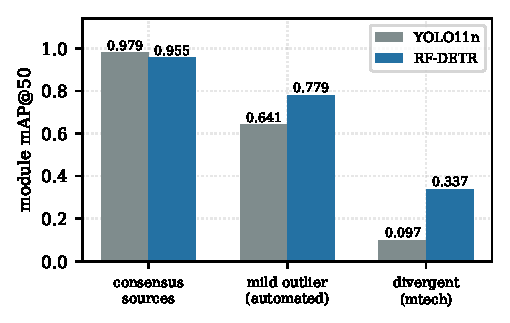
\includegraphics[width=0.98\columnwidth]{figures/fig_arch.pdf}
\caption{Architecture comparison under a matched budget. The self-supervised
pretrained model is marginally weaker on conventionally annotated packs and
substantially stronger on both out-of-convention sources.}
\label{fig:arch}
\end{figure}

The result is narrow and specific. On conventionally annotated packs the
self-supervised pretrained model is marginally \emph{worse}, at 0.955 against 0.979.
On the mild outlier it scores 0.779 against 0.641, and on the divergent source 0.337
against 0.097, an improvement of a factor of 3.5. Self-supervised pretraining
therefore does not detect ordinary modules more accurately in this setting; it
degrades considerably more gracefully when the definition of the target moves. On a
line receiving heterogeneous packs, graceful degradation is the property of practical
value, and the proposed screening procedure and the choice of pretraining are
complementary rather than alternative responses to the same problem.

Both architectures produce the same partition under the screen, flagging the same two
sources, which indicates the screening procedure to be independent of the detector it
is applied to.

\subsection{Single-Source Validation Inverts Checkpoint Selection}
\label{sec:res-inversion}

\noindent A result emerged from the matched-budget runs that was not sought and that
bears directly on the paper's central claim. The validation data available for this
corpus is drawn overwhelmingly from the divergent source. During training, accuracy on
that validation split peaked early and then fell by roughly a factor of five, while
both training losses decreased monotonically throughout. Selecting a checkpoint on
that signal is therefore selecting for the divergent convention.

The consequence is quantified in Table~\ref{tab:inversion} and
Figure~\ref{fig:inversion}. Evaluated across all sources, the checkpoint selected by
validation accuracy is \emph{worse} than the final checkpoint by 0.235 mAP@50, a
relative loss of 51\%. Across three random seeds the final checkpoint attains
$0.696 \pm 0.003$ and the selected checkpoint $0.461 \pm 0.018$, so the effect is 80
times the seed-to-seed spread. On the module class, 500 bootstrap resamples give
95\% intervals of $[0.659, 0.808]$ and $[0.471, 0.626]$, which do not overlap.

\begin{table}[t]
\caption{Effect of selecting a checkpoint against single-source validation data, mAP@50.}
\label{tab:inversion}
\centering
\begin{tabular}{lcc}
\hline
Checkpoint & All sources & Module, 95\% CI \\
\hline
Val-selected & $0.461 \pm 0.018$ & 0.552 [0.471, 0.626] \\
Fixed-budget final & $\mathbf{0.696 \pm 0.003}$ & \textbf{0.735 [0.659, 0.808]} \\
\hline
\end{tabular}
\end{table}

\begin{figure}[t]
\centering
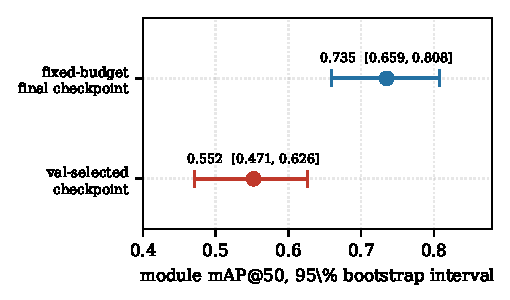
\includegraphics[width=0.98\columnwidth]{figures/fig_inversion.pdf}
\caption{Model selection against single-source validation data. Bars are 95\%
bootstrap intervals over 500 resamples. The checkpoint chosen by validation accuracy
is the worse of the two and the intervals do not overlap.}
\label{fig:inversion}
\end{figure}

The same inversion appears in the self-supervised pretrained model, whose validation
signal identified epoch 3 as best and epoch 60 as substantially worse, while across
sources the epoch-60 checkpoint scores 0.955 against 0.719 on consensus sources and
0.337 against 0.079 on the divergent source. The effect is therefore a property of
single-source validation and not of one architecture.

Two caveats bound the claim. The evaluation sample is drawn from the corpus rather
than held out, so later checkpoints are favoured by memorisation and the absolute size
of the gap is optimistic. What memorisation does not explain is the \emph{pattern}:
memorising would raise the final checkpoint uniformly, whereas it gains on the
consensus sources while losing on the divergent one, which is a convention trade-off
rather than a fitting effect. Secondly, the finding concerns validation data drawn
from a single divergent source and does not generalise to well-constructed validation
splits.

\subsection{Deployment Cost and Zero-Shot Transfer}

\noindent Evaluated on 17 pack families absent from the corpus, drawn from an
unlabelled public collection, the merged-corpus detector attains a mean detection rate
of 0.76 and finds busbars in 16 of the 17, with 1.00 on BMW i4 and Hyundai Ioniq
against 0.27 on a Volvo truck pack. Module geometry therefore transfers to unseen
passenger-vehicle packs, whereas unusual form factors remain the weak axis. It should
be noted that a detection-rate proxy measures recall only and cannot detect false
positives.

Dynamic INT8 quantisation to the ONNX format reduced median CPU latency from
56.3\,ms to 44.8\,ms and file size from 6.3\,MB to 3.4\,MB, for a loss of 0.007
mAP@50, measured as the median over 20 images on an Apple M1 processor with no
graphics acceleration. The detector is therefore deployable without a graphics
processor at approximately 22 frames per second.

\subsection{Negative Results}
\label{sec:negative}

\noindent Five failures constrain the design space for this task. Each is reported
because it was expected to succeed and because the expectation is common in the
surrounding literature.

\textbf{Open-vocabulary detection is unusable for this task.} YOLO-World
\citep{yoloworld}, prompted with \texttt{ev battery module} and \texttt{busbar},
attained 0.004 mAP@50. Battery internals lie too far outside the vision-language
pre-training distribution for the prompts to ground, so the annotation-free route is
not currently available for this application.

\textbf{Naive multi-source merging degrades accuracy.} Training on the merged corpus
without screening reduced module mAP@50 to 0.094 on the single-source test split,
against a single-source baseline of 0.818. More data made the model worse. This result
motivated the screening procedure of Section~\ref{sec:screen} and illustrates that
curation dominates volume when conventions conflict.

\textbf{Automatic relabelling cannot reconcile a divergent convention.} Reconciliation
of the flagged source with the consensus convention was attempted using Grounding DINO
\citep{groundingdino}. On clean frames the model recovered two of approximately five
modules, and on the greyscale macro imagery that dominates the source it produced
boxes covering half the frame. Relabelling 1,756 images on that basis would have
injected substantial noise. Convention conflicts are therefore not cheaply repairable
after collection, which argues for agreeing annotation guidelines before collection.

\textbf{Copy-paste and glare augmentation degrade the detector.} Copy-paste
compositing \citep{ghiasi2021copypaste} combined with a synthetic glare pass was
applied in order to address the specular highlights characteristic of battery
internals. Validation mAP@50 declined monotonically over the first six epochs, from
0.503 to 0.270 against a baseline of 0.818, and training was terminated. The likely
cause is label noise introduced at paste boundaries together with glare intensity that
does not match the statistics of the real bright-condition imagery.

\textbf{Prolonged fine-tuning degrades the self-supervised pretrained model.} Under
the matched 60-epoch budget the pretrained model reached its best validation accuracy
at epoch 3 or 4 in both runs and improved on no subsequent epoch, ending 27\% below
its peak. A model that arrives already fitted to the task gains nothing from a budget
chosen to suit a model trained from scratch, which is a consideration when matching
budgets across architectures.

\section{\uppercase{Discussion}}

\noindent Three practical implications follow from the results presented above.

Firstly, accuracy reported on a single-source benchmark should not be treated as
an estimate of deployment accuracy for this task, and the gap is large enough to
change engineering decisions rather than merely to qualify them. A detector
selected on in-domain accuracy alone would have selected the specialist, which is
the worst of the three configurations on the cross-facility benchmark.

Secondly, when a corpus is assembled from heterogeneous sources, per-source
disaggregated reporting is a requirement rather than an option. An aggregate
figure computed across conventions that disagree describes no realisable
deployment condition. The proposed screening procedure makes the necessary
partition explicit and reproducible, at the cost of a single evaluation pass over
a model that is trained in any case.

Thirdly, the choice of backbone and the curation of the corpus address the same
failure mode by different means, and the results indicate that curation is the
more effective of the two. Screening recovers 0.227 module mAP@50 for YOLO11n,
whereas substituting a self-supervised pretrained backbone recovers 0.133 of that
same loss at substantially greater inference cost. The two are nevertheless
complementary, since a divergent source that has not been identified is still
handled more gracefully by the self-supervised backbone.

\section{\uppercase{Limitations}}
\label{sec:limits}

\noindent The 66\% relative loss reported in Section~\ref{sec:res-gap} is measured
against an in-domain benchmark that is itself the convention-divergent source. The
figure therefore conflates generalisation loss with the specialist having been trained
on an idiosyncratic convention, and it is read as an upper bound on the generalisation
component rather than as a measurement of it. A second in-domain reference source
would separate the two contributions. No other result in this paper depends on it.

Both screens are computed on a stratified sample of the corpus rather than on held-out
data, because the validation split available here spans only two sources and cannot
support a per-source outlier test. Absolute values are consequently optimistic, and
later checkpoints are additionally favoured by memorisation. Only relative orderings
are used, and the inversion of Section~\ref{sec:res-inversion} rests on a pattern that
memorisation does not produce, but a held-out multi-source split would give a cleaner
measurement of the magnitudes.

YOLO11n was trained with three random seeds, giving a standard deviation of 0.003. The
self-supervised pretrained model was trained once at the full budget, for reasons of
compute; a second run reproduced its early-peak behaviour but was halted at epoch 9.
Its numbers therefore carry no variance estimate.

The proposed screening procedure requires that divergent sources are a minority of the
corpus, since the median defines the consensus. It has been validated on a corpus
containing one severely divergent source and one mild case, and would require
modification for a corpus in which two or more mutually incompatible conventions are
each well represented. It also requires a minimum number of instances per source; three
sources in this corpus fall below that floor and are excluded rather than reported.

The benchmark inherits the annotation conventions of its sources and no independently
relabelled gold subset was constructed, so model error and label error cannot be
separated on it. This is a material limitation for a study whose central claim concerns
annotation quality, and its removal is the first item of future work.

The corpus is assembled from public sources rather than collected under controlled
conditions, so pack-type coverage is uneven and licences vary. One source representing
24\% of the training images is licensed CC BY-NC-SA 4.0, whose ShareAlike condition
propagates to any derivative corpus. One further source became unavailable during this
study, which is a reproducibility risk inherent to corpora assembled from public
repositories.

Finally, absolute accuracy on the busbar class remains modest and is not sufficient for
autonomous operation on that class. The results presented here characterise the failure
modes of the task rather than deliver a deployable detector.

\section{\uppercase{Conclusions}}

\noindent This paper presented a cross-facility corpus and benchmark for electric
vehicle battery component detection, and used it to establish that annotation
convention, rather than architecture, is the dominant failure mode in this
application. Per-source accuracy for a single detector spans 0.097 to 1.000, and the
collapse occurs where a source disagrees about what the target class denotes rather
than where the imagery is hard.

The proposed screening procedure identifies such sources from a single training run,
and a training-free variant computed from annotation geometry identifies the same
source with no training at all. Both pass a positive control in which a consensus
source is relabelled to a deliberately different convention: the manipulated source is
recovered by both screens while no other source changes status.

Two results about method rather than data follow. Under a matched training budget,
self-supervised pretraining is marginally worse on conventionally annotated packs and
better by a factor of 3.5 under annotation shift, which narrows the circumstances in
which it should be preferred to graceful degradation rather than accuracy. And
validation data drawn from a single divergent source inverts checkpoint selection: the
selected checkpoint is worse than the fixed-budget final checkpoint by 51\% relative,
with non-overlapping bootstrap intervals, and the same inversion appears in both
architectures tested.

Taken together, these results indicate that dataset design, and specifically agreement
on annotation convention before collection, is the first thing to get right in this
application, and that the same disagreement propagates silently into model selection
if the validation split is not itself checked.

Future work will construct an independently relabelled gold subset in order to
separate model error from label error, will repeat both screens on a held-out
multi-source split, and will extend the training-free index to forms of convention
divergence that preserve object scale.
